\documentclass[12pt, notitlepage]{article}
\usepackage[utf8]{inputenc}
\usepackage{graphicx}
\graphicspath{ {images/} }

\usepackage[english]{babel}
\usepackage[nottoc]{tocbibind}

\usepackage{hyperref}
\usepackage[left=3cm,right=3cm,top=2cm,bottom=2cm]{geometry}

\usepackage{bbm}

\usepackage{amsmath}
\usepackage{amsthm}
\usepackage{amsfonts}
\usepackage{amssymb}
\newtheorem{thm}{Theorem}[section]
\newtheorem{lem}[thm]{Lemma}
\newtheorem{prop}[thm]{Proposition}
\newtheorem{cor}[thm]{Corollary}
\newtheorem{conj}[thm]{Conjecture}
\newtheorem{exmp}[thm]{Example}
\newtheorem{remark}[thm]{Remark}

\usepackage{mathtools}
\usepackage{tikz-cd}

\usepackage{xcolor}

\theoremstyle{definition}
\newtheorem{defn}{Definition}[section]

\title{Proofs of some technical results}
\author{Sayantan Khan}
\date{July 2017}

\usepackage{gentium}

\usepackage{todonotes}

\newcommand{\cat}[1]{\mathrm{#1}}
\newcommand{\cohomtheorie}{{h}^{\ast}}
\newcommand{\calz}{\mathcal{Z}}
\newcommand{\redco}{\widetilde{h}}
\newcommand{\dv}{\mathrm{DV}}
\newcommand{\coker}{\mathrm{coker}}

\makeatletter
\newcommand{\colim@}[2]{%
  \vtop{\m@th\ialign{##\cr
    \hfil$#1\operator@font colim$\hfil\cr
    \noalign{\nointerlineskip\kern1.5\ex@}#2\cr
    \noalign{\nointerlineskip\kern-\ex@}\cr}}%
}
\newcommand{\colim}{%
  \mathop{\mathpalette\colim@{\rightarrowfill@\textstyle}}\nmlimits@
}
\makeatother

\begin{document}
\maketitle

\tableofcontents

% \todototoc \listoftodos

\newpage

\section{Blakers-Massey Theorem}
\label{sec:blak-mass-theor}

Fill in later

\section{Comparison theorem for cohomology theories}
\label{sec:comp-theor-cohom}

Fill in later

\section{Brown's representability theorem}
\label{sec:browns-repr-theor}

In this section, we shall see that all reduced cohomology theories that satisfy the wedge sum
($\dv$) axiom are representable functors, i.e. they are naturally isomorphic to the hom functor in
the homotopy category $\cat{hCW}_{\ast}$. In particular, for a given reduced cohomology theory
$\cohomtheorie$, we'll construct a sequence of spaces $\calz(n)$, which we'll call a spectrum, such
that $\redco^n(X)$ is naturally isomorphic to $\left[X, \calz(n)\right]$.

\subsection{Spectra and cohomology theories}
\label{sec:spectra-cohom-theor}

\begin{defn}[$\Omega$-Spectrum]
  A spectrum is a $\mathbb{Z}$ indexed sequence of pointed spaces $\calz(n)$ together with structure
  maps $\sigma_n: \Sigma \calz(n) \to \calz(n+1)$. If the adjoints of the structure maps, i.e. the
  maps $\widetilde{\sigma}_n: \calz(n) \to \Omega \calz(n+1)$ are homotopy equivalences, then the
  spectrum is called an $\Omega$-spectrum.
\end{defn}

\begin{prop}
  Given a $\Omega$-spectrum $\calz$, one can define the following functor.
  \begin{align*}
    \redco^n(X; \calz) = \left[X, \calz(n)\right]
  \end{align*}
  This is a contravariant functor which satisfies the homotopy invariance $(\mathrm{H})$, suspension
  $(\mathrm{S})$, exactness $(\mathrm{E})$, and the wedge sum $(\dv)$ axiom. It is therefore a
  reduced cohomology theory.
\end{prop}

\begin{proof}
  We'll deal with the axioms one at a time.
  \begin{description}
  \item[Homotopy invariance (H):] This is obvious, because we are looking at homotopy classes of
    maps.
  \item[Suspension (S):] We need to show there is a natural isomorphism from $\redco^n(X)$ to
    $\redco^{n+1}(\Sigma X)$. Note that the adjoint of the structure maps are homotopy equivalences.
    We therefore have a natural isomorphism.
    \begin{align*}
      \left[ X, \calz(n) \right] \cong \left[ X, \Omega \calz(n+1) \right]
    \end{align*}
    On the other hand, since $\Sigma$ are $\Omega$ are adjoints, we have the following natural
    isomorphism.
    \begin{align*}
      \left[ X, \Omega \calz(n+1) \right] \cong \left[ \Sigma X, \calz(n+1) \right]
    \end{align*}
    Composing the two natural isomorphisms, we get our required isomorphism.
  \item[Exactness (E):] We need to show for any cofibration $i: A \hookrightarrow X$, the following
    sequence is exact.
    \begin{align*}
      \redco^n(A) \leftarrow \redco^n(X) \leftarrow \redco^n\left( X/A \right)
    \end{align*}
    Using the cofiber sequence, we get that following sequence is exact.
    \begin{align*}
      [A, \calz(n)] \leftarrow [X, \calz(n)] \leftarrow \left[\left(X/A\right), \calz(n) \right]
    \end{align*}
  \item[Wedge sum (DV):] The functor $[\cdot, \calz(n)]$ satisfies $(\dv)$ axiom. This is fairly
    easy to check. That means $\redco^{\ast}$ satisfies $(\dv)$ axiom.
  \end{description}
\end{proof}

\todo[size=\tiny]{To construct easy examples of spectra, one needs to check that the filtered
  colimits commute with the loop space functor, at least for nice enough spaces.}
% {\color{red} To construct easy examples of spectra, one needs to check that filtered colimits
% commute with the loop space functor, at least for nice enough spaces.}

\subsection{Proof of Brown's representability theorem}
\label{sec:proof-browns-repr}

In the previous section, we saw that if we are given an $\Omega$-spectrum, we can construct a
reduced cohomology theory using the spectrum. Brown's representability theorem is the converse of
the previous theorem, i.e. given a reduced cohomology theory which satisfies the $(\dv)$ axiom, it
can be represented by an $\Omega$-spectrum, which is unique up to homotopy. This theorem is fairly
technical, and will require the use of the theorem on Milnor exact sequence (theorem
\ref{thm-milnor}).

\begin{thm}[Brown's representability theorem]
  Let $\redco^{\ast}$ be a reduced cohomology theory satisfying the $(\dv)$ axiom. Then there is an
  $\Omega$-spectrum $\calz$ such that $\redco^{n}$ is naturally isomorphic to
  $\left[\cdot, \calz(n) \right]$.
\end{thm}

\begin{proof}
  The proof will have two main parts. The first part will involve constructing the spaces $\calz(n)$
  for each $n$ such that there is a natural isomorphism from $\redco^n(X)$ to
  $\left[ X, \calz(n) \right]$ for all CW complexes $X$. The second part will involve constructing
  the structure maps from $\Sigma \calz(n) \to \calz(n+1)$.

  Fix an $n \in \mathbb{Z}$. We will construct the space $\calz(n)$ as a CW complex, using finite
  dimensional skeletons $\calz(n)_k$. For each $k$, we will also pick a cohomology class $c_n(k)$ in
  $\redco^n(\calz(n)_k)$ such that the map
  $d_n^{m}(k): \left[S^m, \calz(n)_k \right] \to \redco^n(S^m)$ is an isomorphism for $m < k$ and
  surjection for $m=k$ \todo[size=\tiny]{Show that this is a group homomorphism for $m \geq 1$}.
  \begin{align*}
    d_n^{m}(k) &: \left[ S^m, \calz(n)_k\right] \to \redco^n(S^m) \\
    d_n^{m}(k) &: [f] \mapsto f^{\ast}(c_n(k))
  \end{align*}
  For $k=0$, we define $\calz(n)_0$ as follows.
  \begin{align*}
    \calz(n)_0 := \bigvee_{\alpha \in \redco^n(S^0)} S_{\alpha}^0
  \end{align*}
  The cohomology group of $\calz(n)_0$ is given by a direct product, since $\redco^n$ satisfies the
  $\mathrm{(DV)}$ axiom.
  \begin{align*}
    \redco^n(Z(n)_0) \cong \prod_{\alpha \in \redco^n(S^0)} \redco^n(S_{\alpha}^0)
  \end{align*}
  Pick the following element as $c_n(0)$.
  \begin{align*}
    c_n(0) := \prod_{\alpha \in \redco^n(S^0)} \alpha
  \end{align*}
  Since $k=0$, we only need to show that $d_n^0(0)$ is a surjection. Pick any
  $\alpha \in \redco^n(S^0)$.  Corresponding to this $\alpha$, there's a copy of $S^0$ sitting
  inside $\calz(n)_0$. Let $f$ be the inclusion map of this copy of $S^0$ into $\calz(n)_0$. Then
  the induced map on cohomology is the projection map on the $\alpha$\textsuperscript{th}
  coordinate, since the cohomology theory satisfies the $(\dv)$ axiom. Applying this induced map on
  $c_n(0)$, we see that in the $\alpha$\textsuperscript{th} coordinate, it has $\alpha$, because of
  the way we defined it.  This shows the map is surjective.

  To prove the induction step, suppose we have defined the space $\calz(n)_k$ and $c_n(k)$ that
  satisfy the required properties. Let $K_k \trianglelefteq \left[ S^k, \calz(n)_k \right]$
  \todo[size=\tiny]{The cofibration probably works if you take a subset of $K_k$ that does not
    contain the constant map} be the kernel of the map $d_n^k(k)$.  We construct the following map.
  \begin{align*}
    \phi_n(k): \bigvee_{x \in K_k} S^k \to \calz(n)_k \vee \bigvee_{y \in \redco^n(S^{k+1})} S^{k+1}
  \end{align*}
  This map is obtained by taking the wedge of maps from $S^k$ to $\calz(n)_k$ which are contained in
  $K_k$.  This is a cofibration \todo[size=\tiny]{Not sure how to show this, or whether this is
    entirely correct. Need to check later}. By the $(\dv)$ axiom, we have the following cohomology
  groups.
  \begin{align*}
    \redco^n \left( \calz(n)_k \vee \bigvee_{y \in \redco^n(S^{k+1})} S^{k+1} \right) = \redco^n(\calz(n)_k) \times \prod_{y \in \redco^n(S^{k+1})} \redco^n(S^{k+1})
  \end{align*}
  From this, we can immediately see that the elements of
  $\redco^n \left( \calz(n)_k \vee \bigvee_{y \in \redco^n(S^{k+1})} S^{k+1} \right)$ of the form
  $(c_n(k), \bullet)$ (where $\bullet$ is any arbitrary element) is in the kernel of
  $\phi_n^{\ast}(k)$.  Define $\calz(n)_{k+1}$ to be the cofiber of the map $\phi_n(k)$, and let the
  map to the cofiber be $b_n(k)$.  By the exactness axiom, we have that the following sequence is
  exact.
  \begin{align*}
    \redco^n(\calz(n)_{k+1}) \xrightarrow{b_n^{\ast}(k)}  \redco^n(\calz(n)_k) \times \prod_{y \in \redco^n(S^{k+1})} \redco^n(S^{k+1})
    \xrightarrow{\phi_n^{\ast}(k)} \prod_{x \in K_k} \redco^n(S^k)
  \end{align*}
  Pick the following element $A \in \prod_{y \in \redco^n(S^{k+1})} \redco^n(S^{k+1})$.
  \begin{align*}
    A := \prod_{\alpha \in \redco^n(S^{k+1})} \alpha
  \end{align*}
  The element $(c_n(k), A)$ lies in the kernel of $\phi_n^{\ast}(k)$, which means it lies in the
  image of $b_n^{\ast}(k)$. We define $c_n(k+1)$ to be a pre-image of $(c_n(k), A)$. Seeing that the
  associated map $d_n^m(k+1)$ is surjective for $m=k+1$ is easy enough. The proof is the same as
  that in the case of $d_n^0(0)$.\todo[size=\tiny]{Maybe write the proof anyways. See if it adds to
    the clarity at all} The trickier part is showing injectivity for $m < k+1$. Since $d_m^n(k)$ is
  a group homomorphism (for $M \geq 1$), for $m \geq 1$, it will suffice to show the kernel is
  trivial.  \todo[size=\tiny]{I'm skipping the proof of the case when $m=0$. I think it should be
    fairly easy once I figure out why the map is a cofibration.}  Pick an element, say $[f]$ in the
  kernel. We need to show that $f$ is a nullhomotopic map. But at each step, we coned off the kernel
  of $d_n^m(m)$. That means $f$ is nullhomotopic. This shows the injectivity and hence the
  isomorphism for $m < k+1$.

  Next, we define $\calz(n)$ the colimit of the following diagram.
  \begin{align*}
    \calz(n)_0 \xhookrightarrow{b_n(0)} \calz(n)_1 \xhookrightarrow{b_n(1)} \calz(n)_2 \xhookrightarrow{b_n(2)} \cdots
  \end{align*}
  Note that $\calz(n)_k$ are CW subcomplexes of $\calz(n)$, in particular, we can appeal to Milnor's
  theorem \ref{thm-milnor}, i.e. the following sequence is exact.
  \begin{align*}
    0 \rightarrow {\lim_{k}}^1 \redco^{n-1} (\calz(n)_k) \rightarrow \redco^{n} (\calz(n)) \rightarrow \lim_{k} \redco^{n} (\calz(n)_k) \rightarrow 0
  \end{align*}
  Furthermore the element $(c(n)_0, c(n)_1, c(n)_2, \ldots)$ lies in
  $\lim_{k} \redco^{n} (\calz(n)_k)$ since we pick $c(n)_{k+1}$ as a preimage of $c(n)_k$. By
  exactness, we get a preimage $c_n$ in $\redco^{n} (\calz(n))$. We define a map
  $d_n^m: [S^m, \calz(n)] \to \redco^{n}(S^m)$ which sends $[f]$ to $f^{\ast}(c_n)$. Because of the
  inductive construction, we know this is an isomorphism for all $m \geq 0$ (To see this, observe
  that a map from a compact space like $S^m$ factors through a finite stage in the colimit
  $\calz(n)$). This can be extended to a natural isomorphism for all finite CW complexes.
  \todo[size=\tiny]{Need to prove this, but can't think of a proof yet.  The five lemma might help}
  Now that we know how to represent the individual functors $\redco^{n}$, we need to construct the
  structure maps from the suspension homomorphism of the cohomology theory. Let $T_n$ be the
  suspension homomorphism from $\redco^n(X)$ to $\redco^{n+1}(\Sigma X)$. If we set $X$ to be
  $\calz(n)$, we have the following homomorphism.
  \begin{align*}
    T_n: \redco^n(\calz(n)) \to \redco^{n+1}(\Sigma \calz(n+1))
  \end{align*}
  But this is equivalent to the following homomorphism.
  \begin{align*}
    \widetilde{T}_n: [\calz(n), \calz(n)] \to [\Sigma \calz(n), \calz(n+1)]
  \end{align*}
  We do the most obvious thing, i.e. apply $\widetilde{T}_n$ to the homotopy class of the identity
  map, and we pick a map to be our structure map from the resulting homotopy class.
  \todo[size=\tiny]{Show that this forms an $\Omega$-spectrum}

\end{proof}

This result enables us to study any reduced cohomology theory by studying its associated spectrum.
This lets us study many cohomology theories that were intractable by the usual methods, e.g.
cobordism, which is represented by the Thom spectrum.

\newpage

\appendix

\section{Definitions and notation}
\label{sec:definitions-notation}

\begin{defn}[Suspension of a pointed space]
  The suspension $\Sigma X$ of a pointed space $X$ is the smash product $S^1 \wedge X$.
\end{defn}

\begin{defn}[Loop space of a pointed space]
  The loop spaces $\Omega X$ of a pointed space $X$ is the set of all pointed maps from $S^1$ to $X$
  with the compact-open topology.
\end{defn}

\begin{defn}[$\lim^1$]
  Let $T$ be the category of towers of abelian groups, i.e. $\mathbb{N}$ indexed set of abelian
  groups $G_i$ with maps $f_i: G_i \to G_{i-1}$, and maps are set of arrows that make the whole
  thing commute \todo[size=\tiny]{Check that this category has enough injectives}. Then $\lim$ is a
  left exact functor from $T$ to $\cat{AbGrp}$, and we define $\lim^1$ to be the first right derived
  functor of $\lim$.
\end{defn}

\section{Some useful lemmas and theorems}
\label{sec:some-useful-lemmas}

\textbf{Note:} Although we state many of the lemmas here for $\cat{TOP}$, they are also true for
$\cat{TOP}_{\ast}$, and the proof is similar.

\begin{lem}
  If $i: A \hookrightarrow X$ is a cofibration (in the category $\cat{TOP}$), then the mapping cone
  $C(i)$ is homotopy equivalent to $X/A$.
\end{lem}

\begin{proof}
  We will first construct the maps to and from $C(i)$ to $X/A$. The maps from $C(i)$ to $X/A$ is the
  map that collapses the cone of $A$ to a point corresponding to $A$ in $X/A$. Now consider a map
  from $H: A \times I$ to $C(i)$, such that $H$ contracts $A$ to a point in $C(i)$, starting from
  the inclusion of $A$ in $X$. Let the map $j$ from $X$ to $C(i)$ be the inclusion map. Since $i$ is
  a cofibration, we can extend $H$ with the initial condition $j$ to a map $J: X \times I \to
  C(i)$. But $J(\cdot, 1)$ collapses $A$ to a point. That means it factors through a $X/A$. This
  gives us a map $k$ from $X/A$ to $C(i)$.

  The fact that these maps are homotopy inverses can be verified \todo[size=\tiny]{Not sure of
    this. Verify later.} using the homotopy $J$.
\end{proof}

\begin{lem}
  In the category $\cat{TOP}$, the following sequence is h-coexact.
  \begin{align*}
    A \xrightarrow{f} B \xrightarrow{i} C(f)
  \end{align*}
  That means for any space $Z$, the following sequence of abelian groups is exact.
  \begin{align*}
    [A, Z] \leftarrow [B,Z] \leftarrow [C(f), Z]
  \end{align*}
\end{lem}

\begin{proof}
  If an element $[c] \in [B,Z]$ goes to $0$ in $[A, Z]$, that means $c \circ f: A \to Z$ is
  nullhomotopic, where $c$ is a representative of $[c]$. But that means there is some function
  $d \in C(f)$ such that $c = d \circ i$. This shows the exactness of the sequence.
\end{proof}

\begin{lem}
  If $K$ is a compact space, let $A_i$ be a sequence of spaces where points are closed, and $A$ is
  the colimit of the following diagram:
  \begin{align*}
    A_0 \hookrightarrow A_1 \hookrightarrow A_2 \hookrightarrow \cdots
  \end{align*}
  where all the embeddings are closed, then a map from $K$ to $A$ factors finitely through some
  $A_i$.
\end{lem}

\begin{proof}
  Let $J = f(K)$ be the compact image of $K$ in $A$. For each set $A_i \setminus A_{i-1}$, pick an
  element $c_i$ of $J$ in the set, if $J$ intersects $A_i \setminus A_{i-1}$. Since $A_i$'s are
  closed, that means the subset $c_i$ has the discrete topology. Furthermore, since points are
  closed, the set $\{\cup c_i\}$ is a closed subset of $J$, hence compact. And compact spaces with
  discrete topology are finite. That means only finitely many $A_i \setminus A_{i-1}$ intersect $J$.
  This means the map factors through at some finite stage.
\end{proof}

% \begin{thm}[Cofiber sequence]
%   Put in result
% \end{thm}

% \begin{lem}[Characterizing cofibrations]
%   If $i: A \hookrightarrow X$ is a closed inclusion, and there is a retract $r: X \to A$, then $i$
%   is a cofibration.
% \end{lem}

% \begin{proof}
%   fill in later
% \end{proof}

\begin{thm}[Alternative characterization of $\lim^1$]
  If $F$ is an object in the tower category, then $\lim^1(F)$ is the cokernel of the following map.
  \begin{align*}
    \alpha_F : \prod_{i \in \mathbb{N}} F_i &\to \prod_{i \in \mathbb{N}} F_i \\
    \alpha_F : (g_0, g_1, g_2, \ldots) &\mapsto \left(g_0 - f_1(g_1), g_1 - f_2(g_2), \ldots \right)
  \end{align*}
\end{thm}

\begin{proof}
  The first step in characterizing ${\lim}^1$ in the following manner is to pick an appropriate
  injective resolution. Let $F$ be a tower of abelian groups and $I$ an injective tower it maps
  into via a monomorphism $m$.
  \[
    \begin{tikzcd}
      F_0 \ar[d, rightarrowtail, "m_0"] & F_1 \ar[swap]{l}{f_1} \ar[d, rightarrowtail, "m_1"] & F_2 \ar[swap]{l}{f_2} \ar[d, rightarrowtail, "m_2"] & F_3 \ar[swap]{l}{f_3} \ar[d, rightarrowtail, "m_3"] & \cdots \ar[swap]{l}{f_4} \\
      I_0 & I_1 \ar[swap]{l}{i_1} & I_2 \ar[swap]{l}{i_2} & I_3 \ar[swap]{l}{i_3} & \cdots \ar[swap]{l}{i_4}
    \end{tikzcd}
  \]

Without losing any generality, we can assume all the maps $i_k$ in $I$ are surjective. Otherwise, we just
replace $I_k$ by $\bigoplus_{j=0}^k I_j$, and have the maps on all but the last coordinate be the identity.
This is important, because we'll need surjectivity of the maps later. We can now construct an injective
resolution of $F$ as the following exact sequence.

\begin{align*}
  0 \xrightarrow{} F \xrightarrow{m} I \xrightarrow{q} \coker(m) \xrightarrow{} 0
\end{align*}
The first derived functor is the homology at $\lim(\coker(m))$ of the following sequence.

\begin{align*}
  0 \xrightarrow{} \lim(F) \xrightarrow{\lim(m)} \lim(I) \xrightarrow{\lim(q)} \lim(\coker(m)) \xrightarrow{} 0
\end{align*}

Now, just like $\alpha_F$ was defined in the statement of the theorem, we define $\alpha_I$ and $\alpha_{\coker(m)}$.
Then we get the following short exact sequence of chain complexes (the rows are exact).

\[
  \begin{tikzcd}
    & 0 \ar[d] & 0 \ar[d] & 0 \ar[d] & \\
    0 \ar[r] & \prod_{i} F_i \ar[r, "m"] \ar[d, swap, "\alpha_F"] & \prod_{i} I_i \ar[r, "q"] \ar[d, swap, "\alpha_I"] & \prod_{i} \coker(m) \ar[r] \ar[d, swap, "\alpha_{\coker(m)}"] & 0 \\
    0 \ar[r] & \prod_{i} F_i \ar[r, "m"] \ar[d] & \prod_{i} I_i \ar[r, "q"] \ar[d] & \prod_{i} \coker(m) \ar[r] \ar[d] & 0 \\
    & 0 & 0 & 0 & 
  \end{tikzcd}
\]
We can apply the snake lemma to get the following long exact sequence.
\[
  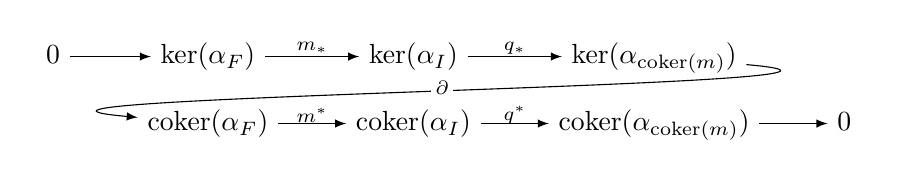
\begin{tikzpicture}[descr/.style={fill=white,inner sep=1.5pt}]
    \matrix (m) [ matrix of math nodes, row sep=1em, column sep=2.5em, text height=1.5ex, text
    depth=0.25ex ]
    { 0 & \ker(\alpha_F) & \ker(\alpha_I) & \ker(\alpha_{\coker(m)}) & \\
     & \coker(\alpha_F) & \coker(\alpha_I) & \coker(\alpha_{\coker(m)}) & 0 \\
    };

    \path[overlay,->, font=\scriptsize,>=latex]
    (m-1-1) edge (m-1-2)
    (m-1-2) edge node[yshift=0.7ex]{$m_{\ast}$} (m-1-3)
    (m-1-3) edge node[yshift=0.7ex]{$q_{\ast}$} (m-1-4)
    (m-1-4) edge[out=355,in=175] node[descr,yshift=0.3ex] {$\partial$} (m-2-2)
    (m-2-2) edge node[yshift=0.7ex]{$m^{\ast}$} (m-2-3)
    (m-2-3) edge node[yshift=0.7ex]{$q^{\ast}$} (m-2-4)
    (m-2-4) edge (m-2-5);
  \end{tikzpicture}
\]
But we see from the definition of $\lim$ that the kernels of $\alpha$ are precisely
the $\lim$. Thus we have the following long exact sequence.
\[
  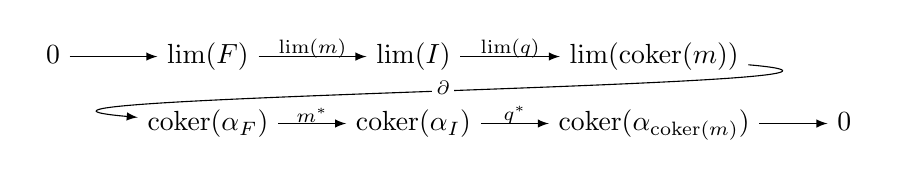
\begin{tikzpicture}[descr/.style={fill=white,inner sep=1.5pt}]
    \matrix (m) [ matrix of math nodes, row sep=1em, column sep=2.5em, text height=1.5ex, text
    depth=0.25ex ]
    { 0 & \lim(F) & \lim(I) & \lim(\coker(m)) & \\
     & \coker(\alpha_F) & \coker(\alpha_I) & \coker(\alpha_{\coker(m)}) & 0 \\
    };

    \path[overlay,->, font=\scriptsize,>=latex]
    (m-1-1) edge (m-1-2)
    (m-1-2) edge node[yshift=0.7ex]{$\lim(m)$} (m-1-3)
    (m-1-3) edge node[yshift=0.7ex]{$\lim(q)$} (m-1-4)
    (m-1-4) edge[out=355,in=175] node[descr,yshift=0.3ex] {$\partial$} (m-2-2)
    (m-2-2) edge node[yshift=0.7ex]{$m^{\ast}$} (m-2-3)
    (m-2-3) edge node[yshift=0.7ex]{$q^{\ast}$} (m-2-4)
    (m-2-4) edge (m-2-5);
  \end{tikzpicture}
\]

The last step in the proof will be to show that $\coker(\alpha_I)$ is $0$, in which
case ${\lim}^1(F)$ is isomorphic to $\coker(\alpha_F)$. Showing that $\coker(\alpha_I)$
is $0$ is equivalent to showing that $\alpha_I$ is surjective. To see this, pick any element
$(j_0, j_1, j_2, \ldots) \in \prod_i I_i$. We need to find an element $(k_0, k_1, k_2, k_3, \ldots)$
such that we have the following equalities.
\begin{align*}
  j_0 &= k_0 - i_1(k_1) \\
  j_1 &= k_1 - i_2(k_2) \\
  j_2 &= k_2 - i_3(k_3) \\
  &\vdots
\end{align*}
But notice that we constructed $I$ such that all the $i_k$ are surjective. That means this system of
equations can be solved simultaneously and $\coker(\alpha_I)$ is $0$. This shows the result.

\end{proof}

\begin{thm}[Milnor exact sequence] \label{thm-milnor} If $\{ i_n : X_n \hookrightarrow X_{n+1} \}$
  for $n \in \mathbb{N}$ are a sequence of nested CW subcomplexes such that $X = \bigcup_n X_n$, and
  $\redco^{\ast}$ is a reduced cohomology theory, then we have the following exact sequence for all
  $i \geq 1$.
  \begin{align*}
    0 \rightarrow {\lim_{n}}^1 \redco^{i-1}(X_n) \rightarrow \redco^i(X) \rightarrow \lim_n \redco^i(X_n) \rightarrow 0
  \end{align*}
\end{thm}

\begin{proof}
  fill in later
\end{proof}

% \bibliography{references} \bibliographystyle{amsplain}

\end{document}
